\section{Experiments on the Lottery Ticket Hypothesis \citep{lottery}}
\label{ap:lottery}
% \vspace{-1ex}

The Lottery Ticket Hypothesis \citep{lottery} conjectures that inside the large network, a sub-network together with their initialization makes the training particularly effective, and together they are termed the ``winning ticket''. In this hypothesis, the original initialization of the sub-network (before large model training) is needed for it to achieve competitive performance when trained in isolation. Their experiments show that training the sub-network with randomly re-initialized weights performs worse than training it with the original initialization inside the large network. In contrast, our work does not require reuse of the original initialization of the pruned model, and shows that random initialization is enough for the pruned model to achieve competitive performance. 

The conclusions seem to be contradictory, but there are several important differences in the evaluation settings: a) Our main conclusion is drawn on \emph{structured} pruning methods, despite for small-scale problems (CIFAR) it also holds on unstructured pruning; \citet{lottery} only evaluates on unstructured pruning. b) Our evaluated network architectures are all relatively large modern models used in the original pruning methods, while most of the experiments in \citet{lottery} use small shallow networks (< 6 layers). c) We use momentum SGD with a large initial learning rate (0.1), which is widely used in prior image classification \citep{resnet, densenet} and pruning works \citep{li2016pruning, liu2017learning, he2017channel, luo2017thinet, he2018sfp, huang2018data} to achieve high accuracy, and is the de facto default optimization setting on CIFAR and ImageNet; while \citet{lottery} mostly uses Adam with much lower learning rates. d) Our experiments include the large-scale ImageNet dataset, while \citet{lottery} only considers MNIST and CIFAR.

\begin{figure*}[!ht]
\centering
\begin{minipage}{0.96\textwidth}
 \begin{subfigure}{\textwidth}
 \centering
 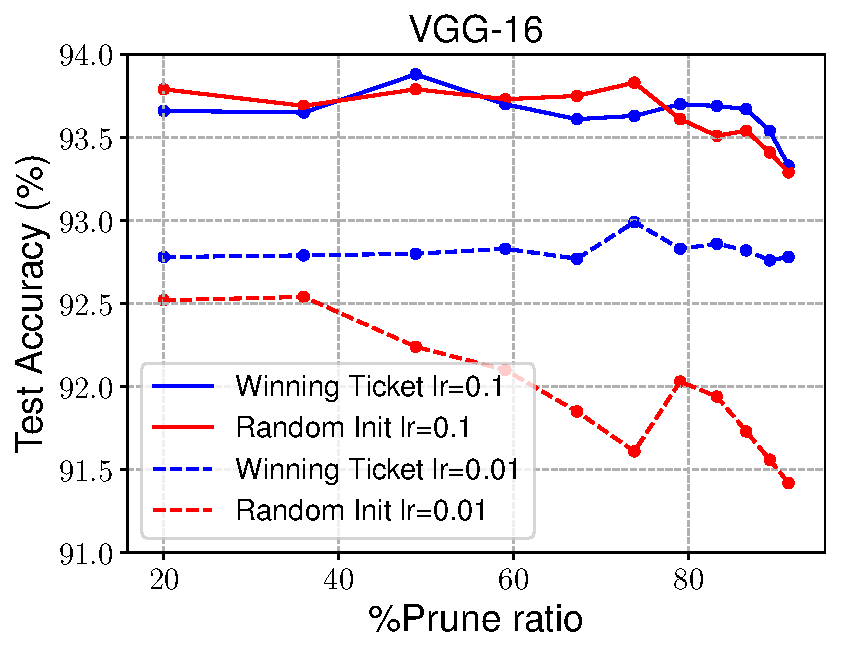
\includegraphics[width=0.47\textwidth]{figures/vgg.pdf}
 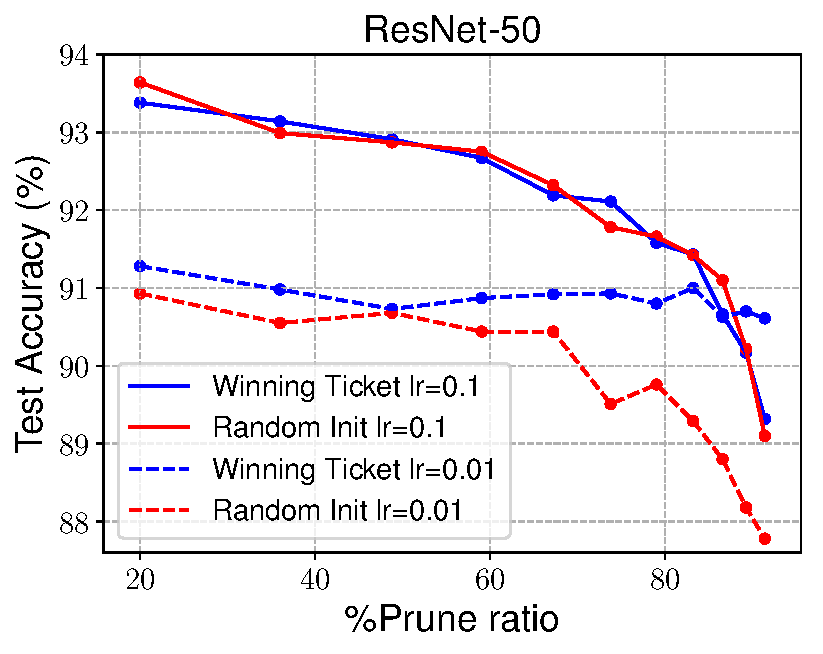
\includegraphics[width=0.46\textwidth]{figures/resnet.pdf}
 \vspace{-2ex}
 \caption{Iterative Pruning}
 \label{iterative-1}
 \end{subfigure}
\end{minipage}
 \begin{minipage}{0.96\textwidth}
 \begin{subfigure}{\textwidth}
 \centering
 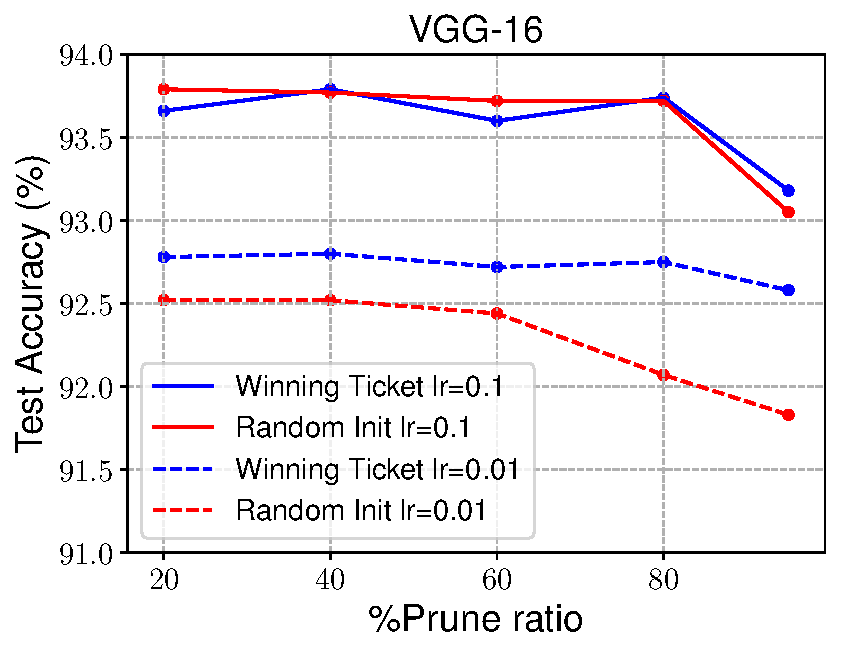
\includegraphics[width=.47\textwidth]{figures/vgg-one-shot.pdf}
 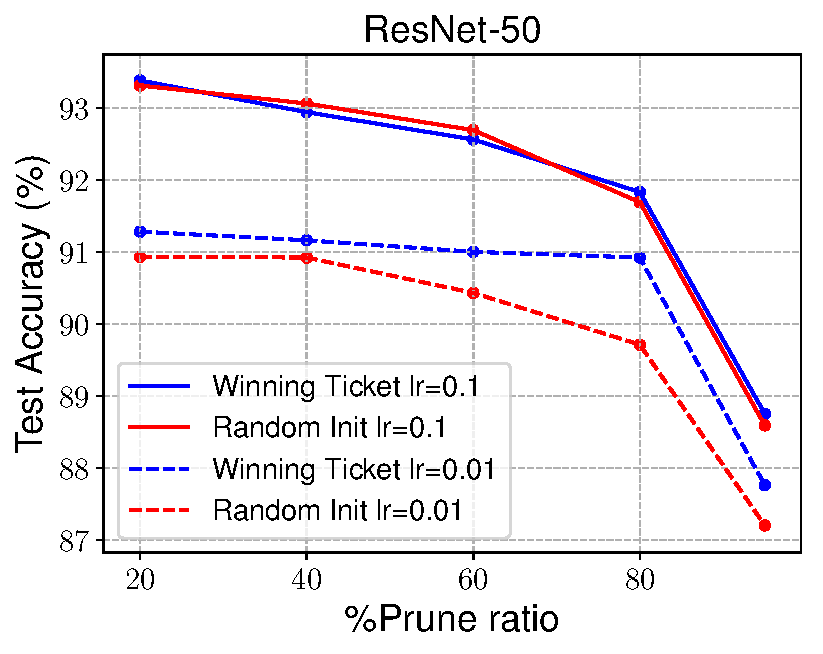
\includegraphics[width=.46\textwidth]{figures/resnet-one-shot.pdf}
 \vspace{-2ex}
 \caption{One-shot Pruning}
 \label{iterative-3}
 \end{subfigure}
\end{minipage}
    \vspace{-1ex}
    \caption{
    Comparisons with the Lottery Ticket Hypothesis \citep{lottery} for iterative/one-shot unstructured  pruning~\citep{han2015learning} with two initial learning rates 0.1 and 0.01, on CIFAR-10 dataset. Each point is averaged over 5 runs. Using the winning ticket as initialization only brings improvement when the learning rate is small (0.01), however such small learning rate leads to a lower accuracy than the widely used large learning rate (0.1).}
    \label{lottery-figure-1}
\end{figure*}



In this section, we show that the difference in learning rate is what causes the seemingly contradicting behaviors between our work and \citet{lottery}, in the case of unstructured pruning on CIFAR. For structured pruning, when using both large and small learning rates, the winning ticket does not outperform random initialization.


\setlength{\tabcolsep}{4pt}
\renewcommand{\arraystretch}{1.15}
\begin{table}[!htbp]
\begin{subtable}[b]{\textwidth}
\centering
\small
\begin{tabular}{c|ccccc}
\hline
Dataset                   & Model                       & Unpruned                     & Pruned Model & Winning Ticket & Random Init \\ \hline
\multirow{5}{*}{CIFAR-10} & VGG-16                      & 93.63 ($\pm$0.16)                  & VGG-16-A     & \textbf{93.62} ($\pm$0.09)  & 93.60 ($\pm$0.15) \\ \cline{2-6} 
                          & \multirow{2}{*}{ResNet-56}  & \multirow{2}{*}{93.14 ($\pm$0.12)} & ResNet-56-A  & 92.72 ($\pm$0.10)  & \textbf{92.75} ($\pm$0.26) \\
                          &                             &                              & ResNet-56-B  & 92.78 ($\pm$0.23)  & \textbf{92.90} ($\pm$0.27) \\ \cline{2-6} 
                          & \multirow{2}{*}{ResNet-110} & \multirow{2}{*}{93.14 ($\pm$0.24)} & ResNet-110-A & \textbf{93.21} ($\pm$0.09)  & \textbf{93.21} ($\pm$0.21) \\
                          &                             &                              & ResNet-110-B & 93.15 ($\pm$0.12)  & \textbf{93.37} ($\pm$0.29) \\ \hline
\end{tabular}
% }
\vspace{2ex}
\caption{Initial learning rate 0.1}
\end{subtable}
\begin{subtable}[b]{\textwidth}
\centering
\small
\begin{tabular}{c|ccccc}
\hline
Dataset                   & Model                       & Unpruned                     & Pruned Model & Winning Ticket & Random Init \\ \hline
\multirow{5}{*}{CIFAR-10} & VGG-16                      &        92.64 ($\pm$0.05)           & VGG-16-A     & 92.65 ($\pm$0.18)  & \textbf{92.67} ($\pm$0.22) \\ \cline{2-6} 
                          & \multirow{2}{*}{ResNet-56}  & \multirow{2}{*}{89.81  ($\pm$0.27)} & ResNet-56-A  & \textbf{90.00} ($\pm$0.15)  & 89.87 ($\pm$0.25) \\
                          &                             &                              & ResNet-56-B  & 89.75 ($\pm$0.35)  & \textbf{89.81} ($\pm$0.24) \\ \cline{2-6} 
                          & \multirow{2}{*}{ResNet-110} & \multirow{2}{*}{89.43 ($\pm$0.39)} & ResNet-110-A & 89.48 ($\pm$0.35)  & \textbf{89.49} ($\pm$0.10) \\
                          &                             &                              & ResNet-110-B & \textbf{89.36} ($\pm$0.30)  & 89.35 ($\pm$0.16) \\ \hline
\end{tabular}
\vspace{2ex}
\caption{Initial learning rate 0.01}
\end{subtable}
\caption{Comparisons with the Lottery Ticket Hypothesis \citep{lottery} on a structured pruning method ($L_1$-norm based filter pruning~\citep{li2016pruning}) with two initial learning rates: 0.1 and 0.01. In both cases, using winning tickets does not bring improvement on accuracy.}
\vspace{-1.5ex}
\label{lottery-2}
\end{table}

We test the Lottery Ticket Hypothesis by comparing the models trained with original initialization (``winning ticket'') and that trained from randomly re-initialized weights. We experiment with two choices of initial learning rate (0.1 and 0.01) with a stepwise decay schedule, using momentum SGD. 0.1 is used in our previous experiments and most prior works on CIFAR and ImageNet. Following \citet{lottery}, we investigate both iterative pruning (prune 20\% in each iteration) and one-shot pruning for unstructured pruning. We show our results for unstructured  pruning~\citep{han2015learning} in \autoref{lottery-figure-1} and \autoref{lottery-1}, and $L_1$-norm based filter pruning~\citep{li2016pruning}  in \autoref{lottery-2}.



\setlength{\tabcolsep}{4pt}
\renewcommand{\arraystretch}{1.15}
\begin{table}[!htbp]
\begin{subtable}[b]{\textwidth}
\centering
\small
\begin{tabular}{c|c|cccc}
\hline
Dataset                    & Model                   & Unpruned          & Prune Ratio & Winning Ticket       & Random Init          \\ \hline
\multirow{10}{*}{CIFAR-10} & \multirow{5}{*}{VGG-16} & \multirow{5}{*}{93.76 ($\pm$0.20)}  & 20\%        & 93.66 ($\pm$0.20)          &   \textbf{93.79} ($\pm$0.11)         \\
                           &                         &               & 40\%        &    \textbf{93.79}  ($\pm$0.12)        &  93.77  ($\pm$0.10)      \\
                           &                         &                & 60\%       &    93.60  ($\pm$0.13)        &   \textbf{93.72} ($\pm$0.11)         \\
                           &                         &               & 80\%       &     \textbf{93.74}  ($\pm$0.15)       & 93.72 ($\pm$0.16)           \\
              &                         &               & 95\%       &     \textbf{93.18}  ($\pm$0.12)       & 93.05 ($\pm$0.21)           \\
                  \cline{2-6} 
                           & \multirow{5}{*}{ResNet-50} & \multirow{5}{*}{93.48 ($\pm$0.20)}    & 20\%        &  \textbf{93.38} ($\pm$0.18)          &      93.31  ($\pm$0.24)             \\
                           &                         &                & 40\%        &     92.94  ($\pm$0.12)                 &  \textbf{93.06} ($\pm$0.22)       \\
                           &                         &                & 60\%        & 92.56 ($\pm$0.20)  & \textbf{92.69}  ($\pm$0.11) \\
                     &                         &               & 80\%        & \textbf{91.83} ($\pm$0.20)  & 91.69 ($\pm$0.21) \\
        &                         &               & 95\%        & \textbf{88.75} ($\pm$0.18)  & 88.59 ($\pm$0.09) \\
                    \hline
\end{tabular}
\vspace{1ex}
\caption{One-shot pruning with initial learning rate 0.1}
\vspace{2ex}
\label{subtable-3}
\end{subtable}
\vspace{2ex}
\begin{subtable}[b]{\textwidth}
\centering
\small
\begin{tabular}{c|c|cccc}
\hline
Dataset                    & Model                   & Unpruned          & Prune Ratio & Winning Ticket       & Random Init          \\ \hline
\multirow{10}{*}{CIFAR-10} & \multirow{5}{*}{VGG-16} & \multirow{5}{*}{92.69 ($\pm$0.12)}  & 20\%        & \textbf{92.78} ($\pm$0.11)           & 92.52 ($\pm$0.15)           \\
                           &                         &             & 40\%        & \textbf{92.80} ($\pm$0.18)           & 92.52 ($\pm$0.15)           \\
                           &                         &               & 60\%       & \textbf{92.72} ($\pm$0.16)           & 92.44 ($\pm$0.19)           \\
 &                         &               & 80\%       & \textbf{92.75} ($\pm$0.07)           & 92.07 ($\pm$0.25)           \\
  &                         &               & 95\%       & \textbf{92.58} ($\pm$0.25)           & 91.83 ($\pm$0.11)           \\ \cline{2-6} & \multirow{5}{*}{ResNet-50} & \multirow{5}{*}{91.06 ($\pm$0.28)}   & 20\%        & \textbf{91.28} ($\pm$0.15)           & 90.93 ($\pm$0.34)           \\
                           &                         &             & 40\%        & \textbf{91.16} ($\pm$0.07)           & 90.92 ($\pm$0.10)           \\
                           &                         &               & 60\%       & \textbf{91.00} ($\pm$0.15)           & 90.43 ($\pm$0.16)           \\
 &                         &               & 80\%       & \textbf{90.92} ($\pm$0.08)           & 89.71 ($\pm$0.18) \\
  &                         &               & 95\%       & \textbf{87.76} ($\pm$0.19)           & 87.20 ($\pm$0.17) \\ \hline
%  & \multirow{4}{*}{VGG-19} & \multirow{4}{*}{92.71 ($\pm$0.17)}   & 20\%        & \textbf{92.67} ($\pm$0.17)           & 92.55 ($\pm$0.20)           \\
%                           &                         &             & 40\%        & \textbf{92.66} ($\pm$0.19)           & 92.64 ($\pm$0.22)           \\
%                           &                         &               & 60\%       & \textbf{92.73} ($\pm$0.24)           & 92.46 ($\pm$0.12)           \\
%  &                         &               & 80\%       & \textbf{92.80} ($\pm$0.19)           & 92.22 ($\pm$0.28)           \\ \hline
\end{tabular}
\vspace{1ex}
\caption{One-shot pruning with initial learning rate 0.01}
\label{subtable-4}
\end{subtable}
\caption{Comparisons with the Lottery Ticket Hypothesis \citep{lottery} for one-shot unstructured  pruning~\citep{han2015learning} with two initial learning rates: 0.1 and 0.01. The same results are visualized in \autoref{iterative-3}. Using the winning ticket as initialization only brings improvement when the learning rate is small (0.01), however such small learning rate leads to a lower accuracy than the widely used large learning rate (0.1).}
\label{lottery-1}
% \vspace{-2ex}
\end{table}





From \autoref{lottery-figure-1} and \autoref{lottery-1}, we see that for unstructured  pruning, using the original initialization as in \citep{lottery} only provides advantage over random initialization with small initial learning rate 0.01. For structured pruning as~\citet{li2016pruning}, it can be seen from \autoref{lottery-2} that using the original initialization is only on par with random initialization for both large and small initial learning rates. In both cases, we can see that the small learning rate gives lower accuracy than the widely-used large learning rate. To summarize, in our evaluated settings, the winning ticket only brings improvement in the case of unstructured pruning, with small initial learning rate, but this small learning rate yields inferior accuracy compared with the widely-used large learning rate. Note that \cite{lottery} also report in their Section 5, that the winning ticket cannot be found on ResNet-18/VGG using the large learning rate. The reason why the original initialization is helpful when the learning rate is small, might be the weights of the final trained model are not too far from the original initialization due to the small parameter updating stepsize.

